%!TEX root = ../tikz-figures.tex

\section*{Graphs}

\index{graph library}
\index{library!graph|see {graph library}}
\index{graph library!poset}
\begin{equation*}
	\begin{tikzpicture}
		\graph[poset=0.7] {
			x0[label=below:$x_0$,x=0.5cm] -- {x01 -- x014[x=1cm], x04},
			x1[label=below:$x_1$] -- {x01, x12 -- x124[x=1cm], x14 -- {x014,x124}},
			x4[label=below:$x_2$, x=-0.5cm] -- {x04 -- x014, x14, x24 -- x124, x34},
			x2[label=below:$x_3$, x=-1cm] -- {x12, x24},
			x3[label=below:$x_4$, x=-0.5cm] -- {x34}
		};
	\end{tikzpicture}
\end{equation*}

\index{brace}
\index{library!calligraphy|see {calligraphy library}}
\index{calligraphy library}
\index{library!decorations|see {decorations library}}
\index{decorations library}
\begin{equation*}
	\begin{tikzpicture}
		\graph[poset] {
			a[x=3cm,label=below:$z$] -- {
				b0 -- c0[x=0.5cm],
				b1 -- {c0, c1[x=0.5cm]},
				b2 -- c1,
				-!- e0[minimum size=0],
				b3 -- c2[x=0.5cm],
				b4 -- {c2, c3[x=0.5cm]},
				b5 -- c3
			}
		};
		\draw (b2) -- ++(0.125,0.25) edge[dotted] +(0.125,0.25);
		\draw (b3) -- ++(-0.125,0.25) edge[dotted] +(-0.125,0.25);
		\node[above=1 of a] {$\cdots$};
		\node[above=1.5 of a] {$\cdots$};
		\draw[decoration={calligraphic brace,amplitude=5pt}, decorate, line width=1.25pt] 
			(0.3,2.3) -- (5.7,2.3);
		\node at (3,2.8) {$2^{k-1}$ top nodes};
	\end{tikzpicture}
\end{equation*}

\begin{equation*}
	\index{every!node}
	\begin{tikzpicture}[ scale=0.5]
		\begin{scope}
			\draw[every node/.style=point] 
				(0,0) node {}
				-- (0,1) node {}
				-- (0,2) node {};
			\node at (0,-1) {${2}$};
		\end{scope}
		\begin{scope}[xshift=80]
			\draw[every node/.style=point] 
				(0,0) node {} -- (-1,1) node {}
				(0,0) -- (0,1) node {}
				(0,0) -- (1,1) node {};
			\node at (0,-1) {${1^3}$};
		\end{scope}
		\begin{scope}[xshift=190]
			\draw[every node/.style=point] 
				(0,0) node {} 
				-- (-1,1) node {} 
				-- (-1,2) node {}
				-- (-1,3) node {}
				(0,0) -- (0,1) node {}
				(0,0) -- (1,1) node {};
			\node at (0,-1) {${3 \cdot 1^2}$};
		\end{scope}
		\begin{scope}[xshift=310]
			\draw[every node/.style=point] 
				(0,0) node {} 
				-- (-1.5,1) node {} 
				-- (-1.5,2) node {}
				-- (-1.5,3) node {}
				(0,0) -- (-0.5,1) node {}
				-- (-0.5,1) node {} 
				-- (-0.5,2) node {}
				-- (-0.5,3) node {}
				(0,0) -- (0.5,1) node {}
				-- (0.5,1) node {} 
				-- (0.5,2) node {}
				(0,0) -- (1.5,1) node {};
			\node at (0,-1) {${3^2 \cdot 2 \cdot 1}$};
		\end{scope}
	\end{tikzpicture}
\end{equation*}

\begin{equation*}
	\begin{tikzpicture}[scale=0.65]
		\begin{scope}
			\graph[poset=0.65] {
				a0[x=1cm] -- {
					b0[y=1.5cm] -- c0[x=1cm,y=3cm],
					b1[y=0.5cm] -- c1[y=1cm] -- c0,
					b2 -- c2 -- {
						c1,
						d1 -- e1 -- {c0, f1[x=0.5cm]},
						d2[y=0.5cm] -- f1
					}
				};
			};
			\node at (1.5,-0.9) {$F$};
		\end{scope}
		\begin{scope}[xshift=120]
			\graph[poset=0.65] {
				a0[x=1cm] -- {
					b0[y=1.5cm] -- c0[x=0.5cm,y=3cm],
					b1[y=0.5cm] -- c1[y=1cm] -- d1[y=2cm],
					b2 -- c2 -- {
						d2[x=-0.5cm] -- e1[x=-0.5cm,y=1cm],
						d3[x=-0.5cm] -- e2[x=-0.5cm] -- {f1[x=-1cm], f2[x=-1cm]},
						d4[x=-1.5cm,y=0.5cm] -- e3[x=-1.5cm,y=1cm]
					}
				};
			};
			\node at (2,-0.9) {$\mathcal T(F)$};
		\end{scope}
		\begin{scope}[xshift=260]
			\graph[poset=0.65] {
				a0[x=2cm] -- {
					b0 -- c0 -- d0 -- e0 -- f0[x=0.5cm],
					b1 -- c1 -- d1 -- e1 -- f1,
					b2[x=1cm] -- c2[x=1cm] -- {
						d2 -- e2 -- f2[x=-0.5cm],
						d3 -- e3 -- {f3[x=-1cm], f4[x=-0.5cm]},
						d4[x=-1cm] -- e4[x=-1cm] -- f5[x=-1cm]
					}
				};
			};
			\node at (2,-0.9) {$T_0$};
		\end{scope}
		\begin{scope}[xshift=420]
			\graph[poset=0.65] {
				a0[x=2cm] -- {
					b0 -- c0 -- d0 -- e0 -- f0[x=1.5cm],
					b1 -- c1 -- d1 -- e1 -- f0,
					b2[x=1cm] -- c2[x=1cm] -- {
						d2 -- e2 -- f0,
						d3 -- e3 -- {f0, f1[x=0.5cm]},
						d4 -- e4 -- f1
					}
				};
			};
			\node at (2,-0.9) {$F'$};
		\end{scope}
	\end{tikzpicture}
\end{equation*}


\begin{equation*}
	\index{graph library!use existing nodes}
	\index{path!curved}
	\begin{tikzpicture}[scale=0.6]
		\node[point] (p) at (0,3) [label=left: $p$] {};
		\node[point] (a0) at (1,2) {};
		\node[point] (c0) at (2,3) {};
		\node[point] (b0) at (3,4) {};
		\node[point] (a1) at (4,3) {};
		\node[point] (c1) at (5,4) {};
		\node[point] (b1) at (6,5) {};
		\node[point] (a2) at (7,4) {};
		\node[point] (q) at (8,5) [label=right:$q$] {};


		\node[point] (d01) at (1,1) {};
		\node[point] (d12) at (4,2) {};
		\node[point] (d11) at (4,1) {};
		\node[point] (d23) at (7,3) {};
		\node[point] (d22) at (7,2) {};
		\node[point] (d21) at (7,1) {};

		\node[point] (r) at (4,-1) [label=below:$p \wedge q$] {};

		% \node[point] (p2) at (0,2) [gray] {};
		% \node[point] (p1) at (0,1) [gray] {};
		% \node[point] (q4) at (8,4) [gray] {};
		% \node[point] (q3) at (8,3) [gray] {};
		% \node[point] (q2) at (8,2) [gray] {};
		% \node[point] (q1) at (8,1) [gray] {};

		\graph[use existing nodes] {
			p -- a0 -- c0 -- b0 -- a1 -- c1 -- b1 -- a2 -- q;
			r -- d01;
			r -- d11;
			r -- d21;
			a0 -- d01;
			a1 -- d12 -- d11;
			a2 -- d23 -- d22 -- d21;
		};
		\draw[gray, out=180, in=230] (r) edge (p);
		\draw[gray, out=0, in=320] (r) edge (q);
	\end{tikzpicture}
\end{equation*}

\begin{equation*}
	\index{path!rounded}
	\index{path!cycle}
	\begin{tikzpicture}
		\begin{scope}
			\graph[poset] {
				a1[x=4cm] -- { 
					b1[x=1cm] -- { 
						c1[x=0.5cm] -- {
							d1 -- {e2[x=0.5cm]},
							d2 -- {e2, e3[x=0.5cm]}
						}, 
						c2 -- d3 -- {e3, e4[x=0.5cm]}
					},
					b2[x=1cm] -- {
						c3 -- d4 -- {e4, e5[x=0.5cm]},
						c4 -- d5 -- {e5, e6[x=0.5cm]},
						c5 -- d6 -- {e6, e7[x=0.5cm]},
					},
					b3 -- c6 -- d7 -- {e7, e8[x=0.5cm]},
					b4 -- c7[x=0.5cm] -- {
						d8 -- {e8, e9[x=0.5cm]},
						d9 -- {e9}
					}
				};
			};
			\draw[dotted,rounded corners=15] (-0.3,4.3) rectangle (8.3,2.7);
			\draw[dashed,rounded corners=20] (4,-0.4) -- (7.3,0.7) -- (8.6,3.35) -- (-0.6,3.35) --  (0.7,0.7) -- cycle;
			\node at (9.3,3.5) {Saw};
			\node at (8.3,1) {Tree};
		\end{scope}
	\end{tikzpicture}
\end{equation*}


\begin{equation*}
	\index{newcommand}
	\index{graph library!custom}
	\index{foreach}
	\index{if statement!ifthenelse}
	\begin{tikzpicture}[xscale=0.9]

		\newcommand{\sawedtreeblock}[1]{
			% \pgfsetmacro\n{#1}
			\begin{scope}[xscale=0.15, yscale=0.4]
				\graph[grow right=0.135cm, empty nodes, nodes={inner sep=0, outer sep=0, minimum size=0}] {
					#1_w_0
						-- #1_a_0[y=1cm]
						-- #1_w_1
						-- #1_a_1[y=1cm]
						-!- #1_e0[minimum size=0]
						-!- #1_ec[x=0.5cm, y=0.25cm, minimum size=0]
						-!- #1_e1[minimum size=0]
						-!- #1_e2[minimum size=0]
						-!- #1_a_{k-2}[y=1cm]
						-- #1_w_{k-1}
						-- #1_a_{k-1}[y=1cm]
						-- #1_w_k
						;
				};
				\node at (#1_ec) {$\cdots$};
				\ifthenelse{\equal{#1}{m}}{
					\node at (5.5,-2) {$F_{m-1}'$};
				}{
					\node at (5.5,-2) {$F_{#1}'$};
				}
				\draw (#1_a_1) -- ++(0.25,-0.25) edge[densely dotted] +(0.5,-0.5);
				\draw (#1_a_{k-2}) -- ++(-0.25,-0.25) edge[densely dotted] +(-0.5,-0.5);
				\ifthenelse{\equal{#1}{m}}{
					\node[point] (#1_z) at (5.5,-5) [label=right:$a_{m-1}$] {};
				}{
					\node[point] (#1_z) at (5.5,-5) [label=left:$a_{#1}$] {};
				}
				\draw (#1_w_0) -- (#1_z) -- (#1_w_k);
			\end{scope}
		}

		\begin{scope}[xshift=-230,yshift=100]
			\sawedtreeblock{0}
		\end{scope}

		\begin{scope}[xshift=-81,yshift=100]
			\sawedtreeblock{1}
		\end{scope}

		\begin{scope}[xshift=100,yshift=100]
			\sawedtreeblock{m}
		\end{scope}

		\begin{scope}[xscale=0.3, yscale=0.4]
			\draw[every node/.style=point] (0_w_k) 
				-- ++(1,1) node (p0_a_0) {}
				-- ++(1,-1) node (p0_w_0) {}
				-- ++(1,1) node (p0_a_1) {}
				-- ++(1,-1) node (p0_w_1)  {}
				-- ++(0.25,0.25)
				edge[densely dotted] +(0.5,0.5)
				++(2.25,0.25) coordinate (p0c)
				++(2.25,0.25)
				edge[densely dotted] +(-0.5,-0.5)
				-- ++(0.25,0.25) node {}
				-- ++(1,-1) node (p0_w_{k-1})  {}
				-- ++(1,1) node (p0_a_{k-1}) {}
				-- (1_w_0);
			\node at (p0c) {$\cdots$};
			\foreach \x in {0,1,{{k-1}}}
			{
				\draw[every node/.style=point] (p0_w_\x)
					-- ++(0,-1) node {}
					-- ++(0,-1) node {}
					-- ++(0,-0.25)
					edge[densely dotted] +(0,-0.5)
					++(0,-1) coordinate (p0_m_\x)
					++(0,-1.5)
					edge[densely dotted] +(0,0.5)
					-- ++(0,-0.25) node (p0_b_\x) {};
				\node at (p0_m_\x) {$\vdots$};
			}
			\draw (p0c) 
				++(0,-2) node {$\cdots$}
				++(0,-2) node {$\cdots$};
		\end{scope}

		\begin{scope}[xscale=0.3, yscale=0.4]
			\draw[every node/.style=point] (1_w_k) 
				-- ++(1,1) node {}
				-- ++(1,-1) node (p1_w_0) {}
				-- ++(0.25,0.25)
				edge[densely dotted] +(0.5,0.5);
			\draw[every node/.style=point] (p1_w_0)
				-- ++(0,-1) node {}
				-- ++(0,-1) node {}
				-- ++(0,-0.25)
				edge[densely dotted] +(0,-0.5)
				++(0,-1) coordinate (p1_m_0)
				++(0,-1.5)
				edge[densely dotted] +(0,0.5)
				-- ++(0,-0.25) node (p1_b_0) {};
			\node at (p1_m_0) {$\vdots$};
			\draw (p1_w_0)
				++(2.5,0.5)
				++(0,-2) node {$\cdots$}
				++(0,-2) node {$\cdots$};
		\end{scope}

		\begin{scope}[xscale=0.3, yscale=0.4]
			\draw[every node/.style=point] (m_w_0) 
				-- ++(-1,1) node {}
				-- ++(-1,-1) node (pm_w_{k-1}) {}
				-- ++(-1,1) node {}
				-- ++(-0.25,-0.25)
				edge[densely dotted] +(-0.5,-0.5);
			\draw[every node/.style=point] (pm_w_{k-1})
				-- ++(0,-1) node {}
				-- ++(0,-1) node {}
				-- ++(0,-0.25)
				edge[densely dotted] +(0,-0.5)
				++(0,-1) coordinate (pm_m_{k-1})
				++(0,-1.5)
				edge[densely dotted] +(0,0.5)
				-- ++(0,-0.25) node (pm_b_{k-1}) {};
			\node at (pm_m_{k-1}) {$\vdots$};
			\draw (pm_w_{k-1})
				++(-2.5,0.5)
				++(0,-2) node {$\cdots$}
				++(0,-2) node {$\cdots$};
		\end{scope}

		\node[point] (z) at (-2,0) [label=below:$\bot$] {};

		\draw (z)
			edge (0_z)
			edge (p0_b_0)
			edge (p0_b_1)
			edge (p0_b_{k-1})
			edge (1_z)
			edge (p1_b_0)
			edge (pm_b_{k-1})
			edge (m_z);

		\begin{scope}[xscale=0.3, yscale=0.4]
			\draw (0_w_0) ++(0,4) node (l0_w_0) {$s_0$};
			\draw (0_w_k) ++(-4,4) node (l0_w_k) {$t_0$};
			\draw (p0_a_0) ++(-2,3) node (lp0_a_0) {$x_{0,0}^*$};
			\draw (p0_w_0) ++(0,4) node (lp0_w_0) {$x_{0,1}^*$};
			\draw (p0_a_1) ++(2,3) node (lp0_a_1) {$x_{0,2}^*$};
			\draw (p0_a_{k-1}) ++(-2,3) node (lp0_a_{k-1}) {$x_{0,k_0}^*$};
			\draw (1_w_0) ++(0,4) node (l1_w_0) {$s_1$};
			\draw (1_w_k) ++(0,4) node (l1_w_k) {$t_1$};
			\draw (m_w_0) ++(0,4) node (lm_w_0) {$s_{m-1}$};
			\draw (m_w_k) ++(0,4) node (lm_w_k) {$t_{m-1}$};
			\draw[-Latex,gray] (l0_w_0) edge (0_w_0);
			\draw[-Latex,gray] (l0_w_k) edge[bend left] (0_w_k);
			\draw[-Latex,gray] (lp0_a_0) edge (p0_a_0);
			\draw[-Latex,gray] (lp0_w_0) edge (p0_w_0);
			\draw[-Latex,gray] (lp0_a_1) edge (p0_a_1);
			\draw[-Latex,gray] (lp0_a_{k-1}) edge (p0_a_{k-1});
			\draw[-Latex,gray] (l1_w_0) edge (1_w_0);
			\draw[-Latex,gray] (l1_w_k) edge (1_w_k);
			\draw[-Latex,gray] (lm_w_0) edge (m_w_0);
			\draw[-Latex,gray] (lm_w_k) edge (m_w_k);
		\end{scope}
			
	\end{tikzpicture}
\end{equation*}


\begin{equation*}
	\begin{tikzpicture}[xscale=0.5,yscale=0.5]
		\begin{scope}
			\draw (0,0) ellipse (3 and 1.1);
			\clip (0,0) ellipse (3 and 1.1);
			\draw (-1.5,-1) -- (-1.5,1);
			\node at (-2,0) {$N$};
			\node[black] at (-0.8,0) {$u_0$};
			\draw[red] (-0.8,0) circle (0.5);
			\node[black] at (0.3,0) {$u_1$};
			\draw[red] (0.3,0) circle (0.5);
			\node[black] at (1.4,0) {$u_2$};
			\draw[red] (1.4,0) circle (0.5);
			\node at (2.5,0) {$\cdots$};
			\coordinate (b000) at (0,-1.2);
			\coordinate (t000) at (0,1.2);
		\end{scope}
		\begin{scope}[xshift=-270,yshift=100]
			\draw (0,0) ellipse (3 and 1.1);
			\clip (0,0) ellipse (3 and 1.1);
			\draw (-1.5,-1) -- (-1.5,1);
			\node at (-2,0) {$N$};
			\node[black] at (-0.8,-0.4) {$u_0$};
			\node[black] at (-0.8,0.4) {$v_0$};
			\draw[blue] (-0.8,0) ellipse (0.5 and 0.9);
			\node[black] at (0.3,0) {$u_1$};
			\draw[red] (0.3,0) circle (0.5);
			\node[black] at (1.4,0) {$u_2$};
			\draw[red] (1.4,0) circle (0.5);
			\node at (2.5,0) {$\cdots$};
			\coordinate (b001) at (0,-1.2);
			\coordinate (t001) at (0,1.2);
		\end{scope}
		\begin{scope}[xshift=-90,yshift=100]
			\draw (0,0) ellipse (3 and 1.1);
			\clip (0,0) ellipse (3 and 1.1);
			\draw (-1.5,-1) -- (-1.5,1);
			\node at (-2,0) {$N$};
			\node[black] at (-0.8,-0.4) {$u_0$};
			\node[black] at (-0.8,0.4) {$v_0$};
			\draw[blue] (-0.8,0) ellipse (0.5 and 0.9);
			\node[black] at (0.3,0) {$u_1$};
			\draw[red] (0.3,0) circle (0.5);
			\node[black] at (1.4,0) {$u_2$};
			\draw[red] (1.4,0) circle (0.5);
			\node at (2.5,0) {$\cdots$};
			\coordinate (b010) at (0,-1.2);
			\coordinate (t010) at (0,1.2);
		\end{scope}
		\begin{scope}[xshift=-90,yshift=200]
			\draw (0,0) ellipse (3 and 1.1);
			\clip (0,0) ellipse (3 and 1.1);
			\draw (-1.5,-1) -- (-1.5,1);
			\node at (-2,0) {$N$};
			\node[black] at (-0.8,-0.4) {$u_0$};
			\node[black] at (-0.8,0.4) {$v_0$};
			\draw[blue] (-0.8,0) ellipse (0.5 and 0.9);
			\node[black] at (0.3,-0.4) {$u_1$};
			\node[black] at (0.3,0.4) {$v_1$};
			\draw[blue] (0.3,0) ellipse (0.5 and 0.9);
			\node[black] at (1.4,0) {$u_2$};
			\draw[red] (1.4,0) circle (0.5);
			\node at (2.5,0) {$\cdots$};
			\coordinate (b011) at (0,-1.2);
			\coordinate (t011) at (0,1.2);
		\end{scope}
		\begin{scope}[xshift=180,yshift=100]
			\draw (0,0) ellipse (3 and 1.1);
			\clip (0,0) ellipse (3 and 1.1);
			\draw (-1.5,-1) -- (-1.5,1);
			\node at (-2,0) {$N$};
			\node[black] at (-0.8,-0.4) {$u_0$};
			\node[black] at (-0.8,0.4) {$v_0$};
			\draw[blue] (-0.8,0) ellipse (0.5 and 0.9);
			\node[black] at (0.3,0) {$u_1$};
			\draw[red] (0.3,0) circle (0.5);
			\node[black] at (1.4,0) {$u_2$};
			\draw[red] (1.4,0) circle (0.5);
			\node at (2.5,0) {$\cdots$};
			\coordinate (b100) at (0,-1.2);
			\coordinate (t100) at (0,1.2);
		\end{scope}
		\begin{scope}[xshift=90,yshift=200]
			\draw (0,0) ellipse (3 and 1.1);
			\clip (0,0) ellipse (3 and 1.1);
			\draw (-1.5,-1) -- (-1.5,1);
			\node at (-2,0) {$N$};
			\node[black] at (-0.8,-0.4) {$u_0$};
			\node[black] at (-0.8,0.4) {$v_0$};
			\draw[blue] (-0.8,0) ellipse (0.5 and 0.9);
			\node[black] at (0.3,-0.4) {$u_1$};
			\node[black] at (0.3,0.4) {$v_1$};
			\draw[blue] (0.3,0) ellipse (0.5 and 0.9);
			\node[black] at (1.4,0) {$u_2$};
			\draw[red] (1.4,0) circle (0.5);
			\node at (2.5,0) {$\cdots$};
			\coordinate (b101) at (0,-1.2);
			\coordinate (t101) at (0,1.2);
		\end{scope}
		\begin{scope}[xshift=270,yshift=200]
			\draw (0,0) ellipse (3 and 1.1);
			\clip (0,0) ellipse (3 and 1.1);
			\draw (-1.5,-1) -- (-1.5,1);
			\node at (-2,0) {$N$};
			\node[black] at (-0.8,-0.4) {$u_0$};
			\node[black] at (-0.8,0.4) {$v_0$};
			\draw[blue] (-0.8,0) ellipse (0.5 and 0.9);
			\node[black] at (0.3,-0.4) {$u_1$};
			\node[black] at (0.3,0.4) {$v_1$};
			\draw[blue] (0.3,0) ellipse (0.5 and 0.9);
			\node[black] at (1.4,0) {$u_2$};
			\draw[red] (1.4,0) circle (0.5);
			\node at (2.5,0) {$\cdots$};
			\coordinate (b110) at (0,-1.2);
			\coordinate (t110) at (0,1.2);
		\end{scope}
		\begin{scope}[xshift=270,yshift=300]
			\draw (0,0) ellipse (3 and 1.1);
			\clip (0,0) ellipse (3 and 1.1);
			\draw (-1.5,-1) -- (-1.5,1);
			\node at (-2,0) {$N$};
			\node[black] at (-0.8,-0.4) {$u_0$};
			\node[black] at (-0.8,0.4) {$v_0$};
			\draw[blue] (-0.8,0) ellipse (0.5 and 0.9);
			\node[black] at (0.3,-0.4) {$u_1$};
			\node[black] at (0.3,0.4) {$v_1$};
			\draw[blue] (0.3,0) ellipse (0.5 and 0.9);
			\node[black] at (1.4,-0.4) {$u_2$};
			\node[black] at (1.4,0.4) {$v_2$};
			\draw[blue] (1.4,0) ellipse (0.5 and 0.9);
			\node at (2.5,0) {$\cdots$};
			\coordinate (b111) at (0,-1.2);
			\coordinate (t111) at (0,1.2);
		\end{scope}
		\draw[->] ($(t000) + (-3,-0.6)$) -- ($(b001) + (2,0.2)$);
		\draw[->] ($(t000) + (-1,0)$) -- ($(b010) + (1,0)$);
		\draw[->] ($(t000) + (2,-0.2)$) -- ($(b100) + (-2,0.2)$);
		\draw[->] (t010) -- (b011);
		\draw[->] ($(t100) + (-1,0)$) -- ($(b101) + (1,0)$);
		\draw[->] ($(t100) + (1,0)$) -- ($(b110) + (-1,0)$);
		\draw[->] (t110) -- (b111);
	\end{tikzpicture}
\end{equation*}

\begin{equation*}
	\index{foreach}
	\index{graph!use existing nodes}
	\begin{tikzpicture}
		\begin{scope}
			\node (a3) at (0,0) {$3$};
			\node (a0) at (-1,1) {$0$};
			\node (a1) at (0,1) {$1$};
			\node (a2) at (1,1) {$2$};
			\graph[use existing nodes] {
				a3 -> {a0,a1,a2},
				a2 -> a1,
				a2 ->[bend right] a0,
				a1 -> a0
			};
			\node at (0,-1) {$(3+1,\ni)$};
		\end{scope}
		\begin{scope}[xshift=100]
			\graph[poset] {
				b000[xshift=1.5cm] -- {
					b001,
					b010 -- {
						b011
					},
					b100[xshift=0.5cm] -- {
						b101,
						b110 -- {
							b111
						}
					}
				}
			};
			\foreach \i in {0,1,2,3}
			{
				\draw (4,\i) -- (4.25,\i) node [label=right:{height $\i$}] {};
			}
			\node at (1.5,-1) {$T_{3}$};
		\end{scope}
	\end{tikzpicture}
\end{equation*}

\begin{equation*}
	\index{calc!relative position}
	\index{arrows!bracket}
	\begin{tikzpicture}[scale=3]
		\node[point] (x) at (-1,0.5) [label=left:$x$] {};
		\node[point] (y) at (0,1) [label=below:$y$] {};
		\node[point] (z) at (1,0.5) [label=right:$z$] {};
		\draw (x) -- (y) -- (z);
		\draw[{[-]}] ($(x)+(0,0.2)$) -- ($(y)+(0,0.2)$) -- ($(z)+(0,0.2)$);
	\end{tikzpicture}
\end{equation*}

\begin{equation*}
	\index{brace!with label}
	\index{node on path!midway}
	\begin{tikzpicture}[xscale=2]
		\node[point] (x) at (-1,0) [label=left:$x$] {};
		\node[point] (y) at (0,0) [label=below:$y$] {};
		\node[point] (z) at (1,0) [label=right:$z$] {};
		\draw (x) -- (y) -- (z);
		\draw[decoration={calligraphic brace,amplitude=5pt}, decorate, line width=1.25pt] ($(x)+(0,0.2)$) -- node [midway, yshift=12] {$[x,y]$} ($(y)+(0,0.2)$);
		\draw[decoration={calligraphic brace,amplitude=5pt}, decorate, line width=1.25pt] ($(y)+(0,0.2)$) -- node [midway, yshift=12] {$[y,z]$} ($(z)+(0,0.2)$);
		\draw[decoration={calligraphic brace,amplitude=5pt}, decorate, line width=1.25pt] ($(z)-(0,0.5)$) -- node [midway, yshift=-12] {$[x,z]$} ($(x)-(0,0.5)$);
	\end{tikzpicture}
\end{equation*}

\begin{equation*}
	\index{path!rounded}
	\index{path!cycle}
	\index{node on path!midway}
	\index{node on path!sloped}
	\index{node on path!fraction position}
	\index{variable!pgfmathsetmacro}
	\index{multiline node text}
	\index{manual scaling}
	\begin{tikzpicture}
		\pgfmathsetmacro{\xscale}{7};
		\pgfmathsetmacro{\yscale}{4};
		\node[align=center] (w) at (0,0) {$\aleph_0$-branch\\well-founded trees};
		\node[align=center] (s) at ({1*\xscale},0) {$\omega$-sequences of\\$\aleph_0$-branch\\well-founded trees};
		\node[align=center] (b) at (0,{1*\yscale}) {branchwise-real\\trees};
		\node[align=center] (q) at ({1*\xscale},{1*\yscale}) {quasi-\\branchwise-real\\trees};
		\node[align=center] (r) at (0,{2.1*\yscale}) {\R-trees};

		\draw[dashed, rounded corners=50] 
			({-0.3*\xscale},{-0.7*\yscale})
			-- ({1.7*\xscale},{1.3*\yscale})
			-- node[above] {Partial orders} ({-0.3*\xscale},{1.3*\yscale})
			-- cycle;
		\draw[dashed] (r) ellipse ({0.2*\xscale} and {0.2*\yscale}) node[above={0.2*\yscale}] {Metric spaces};

		\draw[->] (w) -- node[sloped, above] {$\Road$} (b);
		% \draw[decorate, decoration=snake] (w) -- (s);
		\draw[<->] (w) edge (s);
		\draw[right hook->, bend right=10] (w) edge (q);
		\draw[->] (s) -- node[sloped, above, pos=0.4] {$\Limb$} (q);
		\draw[->] (b) -- node[sloped, below, pos=0.4] {(last week)} (s);
		\draw[->] (b) edge[bend left=10] node[above] {$\Skel$} (q);
		\draw[->] (q) edge[bend left=10] node[below] {$\Fill$} (b);
		\draw[->] (b) edge[bend left] node[rotate=90, above, align=center] {railroad-track} (r);
		\draw[->] (r) edge[bend left] node[rotate=270, above, align=center] {cut-point order} (b);
	\end{tikzpicture}
\end{equation*}


\begin{equation*}
	\index{foreach}
	\index{math functions!trigonmetry}
	\index{limit visualisation}
	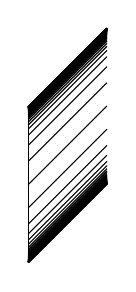
\begin{tikzpicture}
		\foreach \n in {-100,...,100}
		{
			\draw (0,{atan(\n/2)/90}) -- ++(1,1);
		}
		\draw (0,-1) -- (0,1);
	\end{tikzpicture}
\end{equation*}

\begin{equation*}
	\index{multiline node text}
	\index{path!negated}
	\index{path!rounded}
	\index{arrows!double}
	\index{every!node}
	\index{every!path}
	\index{node on path!sloped}
	\begin{tikzpicture}[xscale=4,yscale=1.5,every node/.style={align=center}]

		\node (lR)	at (1,-0.2)	{\R-trees};

		\node (Ra)	at (1,-1)	{(all)};
		\node (Rs)	at (1,-2)	{seperable};
		\node (Rks)	at (1,-3)	{$\kappa$-seperable};
		\node (Rb)	at (1,-4.5)	{boundary-\\countable};
		\node (Rbk)	at (1,-6.5)	{boundary-$\kappa$};

		\node (lB)	at (2.5,-0.2)	{Branchwise-real order trees};

		\node (Pa)	at (2,-1)	{parametrisable};
		\node (Pcb)	at (2,-2)	{parametrisable,\\$\dim(\aleph_1,\aleph_1,\infty)$};
		\node (Pkb)	at (2,-3)	{parametrisable,\\$\dim(\kappa^+,\kappa^+,\infty)$};
		\node (Pct)	at (2,-4)	{parametrisable,\\$\dim(\aleph_1,\aleph_1,\aleph_1)$};
		\node (Pcc)	at (2,-5)	{parametrisable,\\ccc};
		\node (Pkt)	at (2,-6)	{parametrisable,\\$\dim(\kappa^+,\kappa^+,\kappa^+)$};
		\node (Pkc)	at (2,-7)	{parametrisable,\\$\kappa$-cc};

		\node (Ba)	at (3,-1)	{(all)};
		\node (Bcb)	at (3,-2)	{$\dim(\aleph_1,\aleph_1,\infty)$};
		\node (Bkb)	at (3,-3)	{$\dim(\kappa^+,\kappa^+,\infty)$};
		\node (Bct)	at (3,-4)	{$\dim(\aleph_1,\aleph_1,\aleph_1)$};
		\node (Bcc)	at (3,-5)	{ccc};
		\node (Bkt)	at (3,-6)	{$\dim(\kappa^+,\kappa^+,\kappa^+)$};
		\node (Bkc)	at (3,-7)	{$\kappa$-cc};

		\begin{scope}[every path/.style={{To}-{To}}]
			\draw (Ra)	-- (Pa);
			\draw (Rs)	-- (Pcb);
			\draw (Rks)	-- (Pkb);
			\draw (Rb)	-- (Pct);
			\draw (Rb)	-- (Pcc);
			\draw (Rbk)	-- (Pkt);
			\draw (Rbk)	-- (Pkc);
		\end{scope}

		\begin{scope}[every path/.style={double,Implies-Implies}]
			\draw[negated] (Pa)	-- (Ba);
			\draw (Pcb)	-- (Bcb);
			\draw (Pkb)	-- node[above] {\textit{Indep.}} (Bkb);
			\draw (Pct) -- (Pcc);
			\draw (Pct) -- (Bct);
			\draw (Pcc) -- node[above] {\textit{Indep.}} (Bcc);
			\draw (Bct) -- node[above,sloped] {\textit{Indep.}} (Bcc);
			\draw (Pkt) -- (Pkc);
			\draw (Pkt) -- node[above] {\textit{Indep.}} (Bkt);
			\draw (Pkc) -- node[above] {\textit{Indep.}} (Bkc);
			\draw (Bkt) -- node[above,sloped] {\textit{Indep.}} (Bkc);
		\end{scope}

		\draw[dotted,rounded corners=20] (0.6,-0.6) rectangle (1.4,-7.4);

		\draw[dotted,rounded corners=20] (1.6,-0.6) rectangle (3.4,-7.4);
		
	\end{tikzpicture}
\end{equation*}